\documentclass[
    % bleed is added to the final result
    coverheight=9.25in,
    coverwidth=6.125in, % (pagesize - spinewidth) / 2 == (13.042 - 1.042) / 2
    spinewidth=1.042in,
    bleedwidth=0in,
    11pt,
    marklength=0in,
  ]{bookcover}
  
  \usepackage{fancybox}
  \usepackage{wrapfig}
  \usepackage[many]{tcolorbox}
  \usetikzlibrary{calc,positioning, shadings}
  \usepackage[T1]{fontenc}
  \usepackage{fontspec}

  \setmainfont[
    Path=fonts/,
    Extension=.otf,
    UprightFont=*-Regular,
    ItalicFont=*-Italic,
    BoldFont=*-Bold,
    UprightFeatures={SmallCapsFont=*SC-Regular},
    ItalicFeatures={SmallCapsFont=*SC-Italic},
    BoldFeatures={SmallCapsFont=*SC-Bold},
    BoldItalicFeatures={SmallCapsFont=*SC-BoldItalic},
    ]{AlegreyaSans}

  \newcommand{\olpath}{../}
  \newcommand{\whitebg}[1]{%
  \tikz\node[circle,draw,minimum size=1.1cm,
  fill=white,
  path picture={
      \node at (path picture bounding box){
          \includegraphics[width=1.1cm]{\olpath#1}
      };
  }]{};
  }
  \newcommand{\bartosz}{
    \vspace{0pt}
    \begin{tcolorbox}[beamer,
      width=3.6cm,
      arc=0pt,
      boxsep=0pt,
      left=0pt,right=0pt,top=0pt,bottom=0pt,
      ] 
\includegraphics[width=3.6cm]{bartosz}
    \end{tcolorbox}
  }
  \input{\olpath/version}
  
  \definecolor{BackgroundColor}{HTML}{f3f6ed}
  \definecolor{SpineBackColor}{HTML}{262626}
  
  \begin{document}
  
  \begin{bookcover}
    \bookcovercomponent{color}{bg whole}{color=BackgroundColor}
    \bookcovercomponent{color}{spine}{color=SpineBackColor}
    \bookcovercomponent{normal}{front}{
    \newcommand{\stripskip}{4}
\newcommand{\stripwidth}{3}

\begin{tikzpicture}[
    overlay,
    remember picture,
    ribbon/.style={anchor=center, rotate = 45,
                            font={\fontsize{22}{1}\selectfont\bfseries}}
                    ]
    \coordinate (A) at ($ (current page.south east) + (-\stripskip,0) $);% <-- changed coordinate from 'north' to south'
    \coordinate (A') at ($(A) + (-\stripwidth,0) $);

    \coordinate (B) at ($ (current page.south east) + (0,\stripskip) $);% <-- changed coordinate from 'north' to south' and sign for \stripskip
    \coordinate (B') at ($(B) + (0,\stripwidth) $);% <-- changed sign for \stripskip 

    \fill [red!20] (A) -- (A') -- (B') -- (B) -- cycle;

    \coordinate (tempA) at ($(A)!.5!(A')$);
    \coordinate (tempB) at ($(B)!.5!(B')$);

    \node [ribbon](text) at ($(tempA)!.5!(tempB)$) {
        \raisebox{-.30\height}{
\includegraphics[width=.8cm]{\olpath/fig/icons/scala}}
        \hspace{.5mm} Scala Edition
    };

\end{tikzpicture}
    \vspace{1.1cm}
    \begin{center}
      \fontsize{40pt}{5em}\selectfont\bfseries
          CATEGORY THEORY \\FOR PROGRAMMERS
      \vfil
      \hspace*{-.8cm}
\includegraphics[width=.5\coverwidth]{piggie}
      \linebreak
      \rule[1.5cm]{\textwidth/2}{.5pt}\\
      \vspace{-1.5cm}
      \normalfont\Huge\textbf{Bartosz Milewski}
      \vfil
      \vspace*{1cm}
    \end{center}}
    
    \bookcovercomponent{center}{spine}{
      \rotatebox[origin=c]{-90}{\color{orange}
      \Huge\bfseries Category Theory for Programmers \hspace{2em} Bartosz Milewski}}

    \bookcovercomponent{normal}{back}{%
    \begin{minipage}[b][\coverheight][t]{\coverwidth}
      \begin{center}
        \vspace{1cm}
        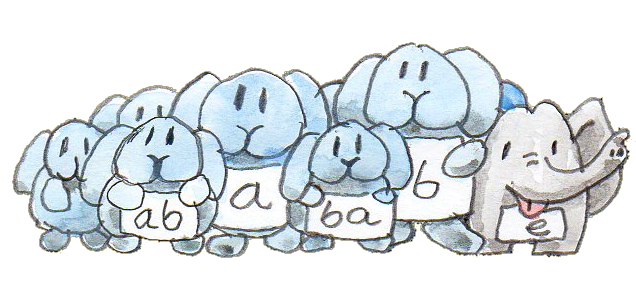
\includegraphics[width=.8\coverwidth]{bunnies}
        \begin{minipage}[t]{.75\coverwidth}
          % Blurb on back cover, gets included in lulu cover as well
% as regular version, so be careful with formatting

{
\parindent=0pt
\parskip=\baselineskip
{\OPTbacktitlefont
\textit{From the Introduction:}}
\OPTbackfont

\emph{Homotopy type theory} is a new branch of mathematics that combines aspects of several different fields in a surprising way. It is based on a recently discovered connection between \emph{homotopy theory} and \emph{type theory}.
It touches on topics as seemingly distant as the homotopy groups of spheres, the algorithms for type checking, and the definition of weak $\infty$-groupoids.

Homotopy type theory brings new ideas into the very foundation of mathematics.
On the one hand, there is Voevodsky's subtle and beautiful \emph{univalence axiom}.
The univalence axiom implies, in particular, that isomorphic structures can be identified, a principle that mathematicians have been happily using on workdays, despite its incompatibility with the ``official'' doctrines of conventional foundations.
On the other hand, we have \emph{higher inductive types}, which provide direct, logical descriptions of some of the basic spaces and constructions of homotopy theory: spheres, cylinders, truncations, localizations, etc.
Both ideas are impossible to capture directly in classical set-theoretic foundations, but when combined in homotopy type theory, they permit an entirely new kind of ``logic of homotopy types''.

This suggests a new conception of foundations of mathematics, with intrinsic homotopical content, an ``invariant'' conception of the objects of mathematics --- and convenient machine implementations, which can serve as a practical aid to the working mathematician.
This is the \emph{Univalent Foundations} program.

The present book is intended as a first systematic exposition of the basics of univalent foundations, and a collection of examples of this new style of reasoning --- but without requiring the reader to know or learn any formal logic, or to use any computer proof assistant.
We believe that univalent foundations will eventually become a viable alternative to set theory as the ``implicit foundation'' for the unformalized mathematics done by most mathematicians.

\bigskip

\begin{center}
  {\Large
  \textit{Get a free copy of the book at HomotopyTypeTheory.org.}}
\end{center}
}

          \vspace{0.6cm}
        \end{minipage}
        
        \begin{minipage}{.85\textwidth}
          \rule{\textwidth}{.5pt}

          \begin{tabular}[h]{p{3.4cm} p{\textwidth}}
            \vspace{5pt}
            \bartosz
            &
            \vspace{10pt}
            \begin{minipage}[b]{.58\coverwidth}
              \fontsize{11pt}{1.4em}\selectfont\textit{Category Theory for Programmers}
                is a series of blog posts by Bartosz Milewski, originally posted on bartoszmilewski.com.\\
                Edited by Igal Tabachnik. Licenced under CC BY-SA 4.0.\\
          \end{minipage}
        \end{tabular}
        \begin{flushright}
          \vspace{-2.6cm}
          \begin{minipage}[b]{4cm}
          \raggedleft
          \whitebg{fig/icons/by}
          \whitebg{fig/icons/cc}
          \whitebg{fig/icons/sa}
          \centering\footnotesize{\texttt{\OPTversion}}
          \end{minipage}
        \end{flushright}
      \end{minipage}
    \end{center}
  \end{minipage}
  }
  \end{bookcover}
\end{document}